\documentclass[mathserif, aspectratio=169]{beamer}
%
%%%%%%%%%%%%%%%%%%%%%%%%%%%%%%%%%%%%%%%%%%%%%%%%%%%%%%%%%%%%%%%%%%%%%%%%
% need to split the includes to make spell checking work.
\usepackage{arev, arevmath}
\usepackage[scaled]{cabin}
\usepackage[T1]{fontenc}
\usepackage[super]{nth}
\usepackage{pifont}
\usepackage{wasysym}
\usepackage{tabularx}
\usepackage{array}
\usepackage{booktabs}
\usepackage{boldline}
\usepackage{colortbl}
%\usepackage{amsmath}
\usepackage{bm}
\usepackage{tcolorbox}
\usepackage{adjustbox}
\usepackage{minibox}
\usepackage{makecell}
\usepackage{adjustbox}
\usepackage{textcomp}
\usepackage[absolute,overlay]{textpos}
\setlength{\TPHorizModule}{1mm}%
\setlength{\TPVertModule}{1mm}%
\tcbuselibrary{skins}

\makeatletter
\newcommand{\antsize}{\@setfontsize{\antsize}{4pt}{4pt}}
\makeatother
\newcommand{\at}{\makeatletter @\makeatother}

\newcommand{\cmark}{\ding{51}}%
\newcommand{\bottomline}[1]{\vskip0pt plus 1fill{\alert{#1}\phantom{g}\vskip 1.0mm}}

\newcommand{\Quote}[2]{%
	\begin{center} 
		\begin{minipage}{0.7\textwidth} 
			\hrule
			\vskip 3mm
			\emph{{\color{ICTPblue} ``#1''}
			
			~~~~ {\color{ICTPorange} --- #2}}
			\vskip 3mm
			\hrule
			\vskip 2mm
		\end{minipage}
	\end{center}}


\mode<presentation>%
{
	\usetheme{default}
	%\usetheme[width=2.5cm]{PaloAlto}
	\usecolortheme{dove}
	\useoutertheme{infolines}
	% oder auch nicht

	% ICTP Colors
	\definecolor{ICTPblue}{RGB}{37,86,162} % 0x255682
	\definecolor{ICTPorange}{RGB}{255,130,0} % 0xff8200
	\definecolor{ICTPgreen}{RGB}{0,100,0}
	\definecolor{ICTPdark}{RGB}{80,80,80} % 0x505050
	\definecolor{ICTPlight}{RGB}{120,120,120}
	\definecolor{ICTPbrown}{RGB}{178,91,0}

	\definecolor{codebg}{rgb}{0.95,0.95,0.95}

	% Color theme
	\setbeamercolor{alerted text}{fg=ICTPorange}
	\setbeamercolor{frametitle}{fg=ICTPblue}
	\setbeamercolor{title}{fg=ICTPblue}
	\setbeamercolor{subtitle}{fg=ICTPorange}
	\setbeamercolor{normal text}{fg=ICTPdark}
	\setbeamercolor{author in foot}{fg=ICTPblue}
	\setbeamercolor{item}{fg=ICTPblue}
	\setbeamercolor{footline}{fg=ICTPblue}
	%\setbeamercolor{item projected}{bg=ICTPorange}
	%\setbeamercolor{item projected}{fg=white}

	\setbeamertemplate{headline}
	{}
	\setbeamertemplate{frametitle}
	{
		%\textbf{{\insertframetitle\phantom{g}}}\\
		%\textbf{\insertframetitle\phantom{g}}\\
		\textbf{\underline{\insertframetitle\phantom{g}}}\\
		%\textbf{\underline{\insertframetitle}}\\
		\vskip 1.0mm
		%{\color{UOLgold}\hrule height 2pt}
		%\par
	}
	\addtobeamertemplate{frametitle}{}{\vspace{-1em}}
	\setbeamertemplate{footline}{
		{%
			\textbf{ \hskip 3.0mm\insertshorttitle\phantom{.}---\phantom{.}\insertshortinstitute\hfill\insertframenumber\,/\,\inserttotalframenumber\hskip 3.0mm} 
		}
	}

	\setbeamertemplate{navigation symbols}{}%remove navigation symbols
	\setbeamertemplate{itemize items}[circle]
	\setbeamertemplate{enumerate items}[fg=ICTPblue]
	\setbeamercolor{itemize items}{fg=ICTPblue}
	\setbeamercolor{sidebar}{bg=ICTPblue}
	\setbeamercolor{title in sidebar}{fg=ICTPorange}
	\setbeamercolor{author in sidebar}{fg=ICTPorange}
	\setbeamercolor{section in sidebar}{fg=ICTPorange}
}

%\input{tikz/common-styles}

\usepackage{graphicx}
\usepackage[latin1]{inputenc}

\graphicspath{{../figs/}{../figs/common/}{../figs/islr/}}

\title[Statistical Learning] % (optional, nur bei langen Titeln n�tig)
{\textbf{Introduction to Statistical Learning\\ {\it with applications in Python}}\\%
		\href{www.statlearning.com}%
		{\tiny\it Based on ``Introduction to Statistical Learning, with applications in R'' by Gareth James, Daniela Witten, Trevor Hastie, Robert Tibishirani}\vspace{2em}}
		\vspace{-2.5cm}{}


		\author{\href{mailto:?to=Kurt Rinnert <kurt.rinnert@cern.ch>&subject=PWF Statistical Learning}{Kurt Rinnert}}

\institute[{\href{https://www.ictp.it/physics-without-frontiers.aspx}{Physics Without Frontiers} --- \href{https://www.ictp.it/}{ICTP}}] % (optional)
{\color{ICTPblue}\bfseries \href{https://www.ictp.it/physics-without-frontiers.aspx}{Physics Without Frontiers}\\\vspace{1mm}%
\href{https://www.ictp.it/}{
\includegraphics[width=0.20\textwidth]{common/ICTP-logo-full-trans.png}}\\%
\href{https://www.liverpool.ac.uk/physics/}{
\includegraphics[width=0.2\textwidth]{common/uol_logo.png}}}

\date{}

\titlegraphic{
	\texorpdfstring{\vspace{-2.8cm}}{}
	 \begin{minipage}[b][1.3cm][b]{0.26\textwidth}\color{ICTPlight}\antsize
		Copyright \textcopyright~2019\\
		\href{mailto:?to=Kurt Rinnert <kurt.rinnert@cern.ch>&subject=PWF Statistical Learning}{Kurt Rinnert <kurt.rinnert{\tt @}cern.ch>},
		\href{mailto:?to=Kate Shaw <kshaw@ictp.it>&subject=PWF Statistical Learning}{Kate Shaw <kshaw{\tt @}ictp.it>}\\
		Copying and distribution of this file, with or without modification,
		are permitted in any medium without royalty provided the copyright
		notice and this notice are preserved.  This file is offered as-is,
		without any warranty.


		Some of the figures in this presentation are taken from ``An Introduction to
		Statistical Learning, with applications in R''  (Springer, 2013) with
		permission from the authors: G. James, D. Witten,  T. Hastie and R. Tibshirani 
	 \end{minipage}\hspace{10cm}
}


\addtocounter{framenumber}{-1}

% nicer table row separation
\renewcommand{\arraystretch}{1.2}

% color boxes
\newcommand{\tabboxset}{\tcbset{enhanced, nobeforeafter, boxrule=0pt, boxsep=0pt, colback=codebg, colframe=codebg, coltext=ICTPdark, rounded corners, arc=4pt, fonttitle={\bfseries\tiny}}}
\newcommand{\codeboxset}{\tcbset{enhanced, nobeforeafter, boxrule=0pt, boxsep=0pt, colback=codebg, colframe=codebg, coltext=ICTPdark, rounded corners, arc=4pt, fonttitle={\bfseries\tiny}}}

\newcommand{\orange}{\color{ICTPorange}}
\newcommand{\blue}{\color{ICTPblue}}
\newcommand{\dark}{\color{ICTPdark}}
\newcommand{\R}{\mathbb{R}}
\newcommand{\dat}[1]{{\footnotesize\tt\orange #1}}
\newcommand{\e}[1]{\emph{#1}}
\newcommand{\bh}{\hat{\beta}}
\newcommand{\h}{\hat}

\makeatletter
\newcommand{\includegraphicsdpi}[3]{%
	\pdfimageresolution=#1%
	\includegraphics[#2]{#3}%
	\pdfimageresolution=72%
}

\newenvironment{blurb}%
	{\begin{center}\begin{minipage}{0.6\textwidth}\footnotesize}
	{\end{minipage}\end{center}}

\newenvironment{cpage}%
	{\begin{center}\begin{minipage}{0.75\textwidth}}
	{\end{minipage}\end{center}}

\newenvironment{popblock}[2]%
	{\begin{center}\begin{minipage}{#1}\footnotesize
		\begin{tcolorbox}[colframe=codebg, colback=white, colupper=ICTPdark, title={\normalsize\bfseries\blue #2}]}
	{\end{tcolorbox}\end{minipage}\end{center}}
\makeatother

\subtitle{\bfseries%
  {Linear Regression, Part 1}\\%
  {\tiny\it linear models, least square fit, simple linear regression, parameter \& model accuracy}\\%
}
\begin{document}
\frame[plain]{
	\vskip 1.0mm
	\titlepage
	\vskip 1.0mm
}


\begin{frame}{Abstract}

	\begin{blurb}
		Linear models are an important topic in statistical learning.  

		The true relationships between predictors and responses are rarely linear.
		But linear models often provide reasonable approximation. They provide
		high interpretability and have low variance, mitigating the risk of over-fitting.
		Linear models can be extended to include (some) non-linear relationships. 

		Linear models also provide an excellent baseline to compare other models against: if 
		our sophisticated model does not do much better than a linear model we might consider
		trading some bias for lower variance.
	\end{blurb}
\end{frame}

\begin{frame}{Overview}
	\begin{itemize}
		\item Linear models with one predictor.
		\item Least squares fit.
		\item Accuracy of parameter estimates.
		\item Model Accuracy.
	\end{itemize}
	\bottomline{This will require some mathematics.}
\end{frame}

\begin{frame}{The Advertising Data Set}
	\begin{center}
		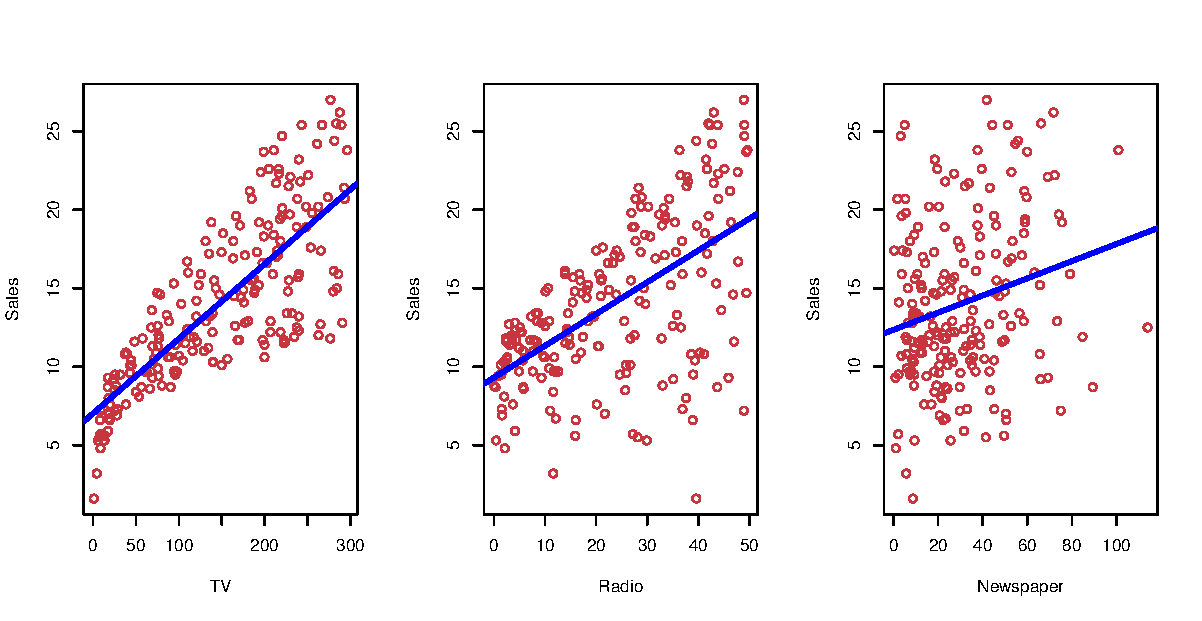
\includegraphics[width=0.6\textwidth]{2_1}

		We want to understand how \dat{sales} depends on \dat{TV}, \dat{radio} and \dat{newspaper}.
	\end{center}
	\bottomline{We will use this data set to illustrate the concepts in this lecture.}
\end{frame}

\begin{frame}{Interesting Questions}
	\begin{enumerate}
		\item Is there a relationship between advertising budget and sales?
		\item How strong is the relationship between advertising budget and sales?
		\item Which media contribute to sales?
		\item How accurately can we estimate the effect of each medium on sales?
		\item How accurately can we predict future sales?
		\item Is the relationship linear?
		\item Is there synergy among the advertising media?
	\end{enumerate}
	\bottomline{Linear regression can answer all of these questions.}
\end{frame}

\begin{frame}{Simple Linear Regression}
	\begin{itemize}
		\item Simple linear regression assumes an approximate simple linear relationship between\\
			one predictor and the response:
			\[ Y \approx \beta_0 + \beta_1 X \]
		\item For example, $X$ might represent the \dat{TV} budget and $Y$ might represent \dat{sales}:
			\[ \text{\dat{sales}} \approx \beta_0 + \beta_1\times\text{\dat{TV}} \]
		\item The \e{coefficients}, or \e{parameters}, $\beta_0$ and $\beta_1$ are the \e{intercept} and
			\e{slope} of a line.
		\item We can \e{estimate} the parameters from the training data and \e{predict} \dat{sales}\\
			from the \dat{TV} budget.
			\[ \hat{y} = \hat{\beta}_0 + \hat{\beta}_1 x \]
	\end{itemize}
	\bottomline{We use the \e{hat} symbol, $\;\bm{\hat{}}\;$, to denote estimates and predictions.}
\end{frame}

\begin{frame}{Estimating the Coefficients}
	\begin{itemize}
		\item In practice, $\beta_0$ and $\beta_1$ are unknown.
		\item Given the training data 
			\[ (x_1, y_1), (x_2, y_2), \dots, (x_n, y_n) \]
			we want to obtain estimates of the coefficients $\beta_0$ and $\beta_1$ such that
			\[ y_i \approx \hat{\beta}_0 + \hat{\beta}_1 x_i,\;\; \forall i = 1,\dots,n \]
		\item In other words we want to find $\hat{\beta}_0$ and $\hat{\beta}_1$ such that the
			resulting line is as close\\
			as possible to the $n = 200$ observations in the \dat{Advertising} data set.
	\end{itemize}
	\bottomline{We need to define what we mean by ``close''.}	
\end{frame}

\begin{frame}{Residual Sum of Squares}
	\begin{itemize}
		\item Given the predictions of $Y$ for the $i$th value of $X$
			\[ \hat{y}_i = \hat{\beta}_0 + \hat{\beta}_1 x_i \]
			we define the $i$ith \e{residual} as
			\[ e_i = y_i - \hat{y}_i \]
		\item The \e{residual sum of squares} is then
			\[ \text{RSS} = e_1^2 + e_2^2 + \dots + e_n^2 \]  
			or equivalently
			\[ \text{RSS} 
				= (y_1 - \hat{\beta}_0 - \hat{\beta}_1 x_1)^2 
				+ (y_2 - \hat{\beta}_0 - \hat{\beta}_1 x_2)^2
				+ \dots
				+ (y_n - \hat{\beta}_0 - \hat{\beta}_1 x_n)^2\] 
	\end{itemize}
	\bottomline{A least squares fit minimises the RSS.}
\end{frame}

\begin{frame}{Least Squares Fit}
	\begin{itemize}
		\item The \e{least squares} approach chooses $\hat{\beta}_0$ and $\hat{\beta}_1$
			to minimise the RSS.
		\item Using some calculus and sum manipulation we can show that the optimal\\
			parameter estimates are:
				\begin{align*}
					\hat{\beta}_1 &= \frac{\sum_{i=1}^n (x_i - \overline{x})(y_i - \overline{y})}
					{\sum_{i=1}^n (x_i - \overline{x})^2}\\
					\phantom{a} & \phantom{b} \\
					\hat{\beta}_0 &= \overline{y} - \hat{\beta}_1 \overline{x}\\
				\end{align*}
	\end{itemize}
	\bottomline{Buckle up, we are going to prove it on the blackboard.}
\end{frame}

\begin{frame}{Least Squares Fit}
	\begin{center}
		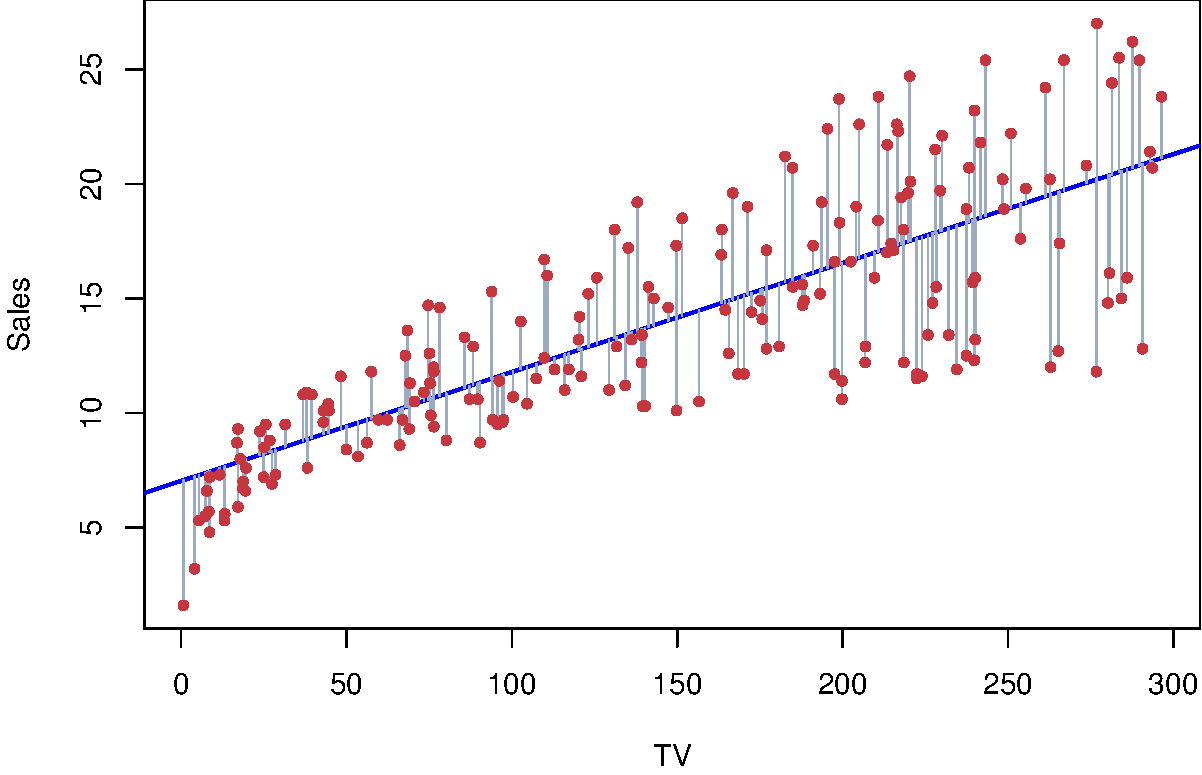
\includegraphics[width=0.6\textwidth]{3_1}

		Result of the least squares fit for the regression of \dat{sales} onto \dat{TV}.
	\end{center}
\end{frame}

\begin{frame}{Least Squares Fit}
	\begin{center}
		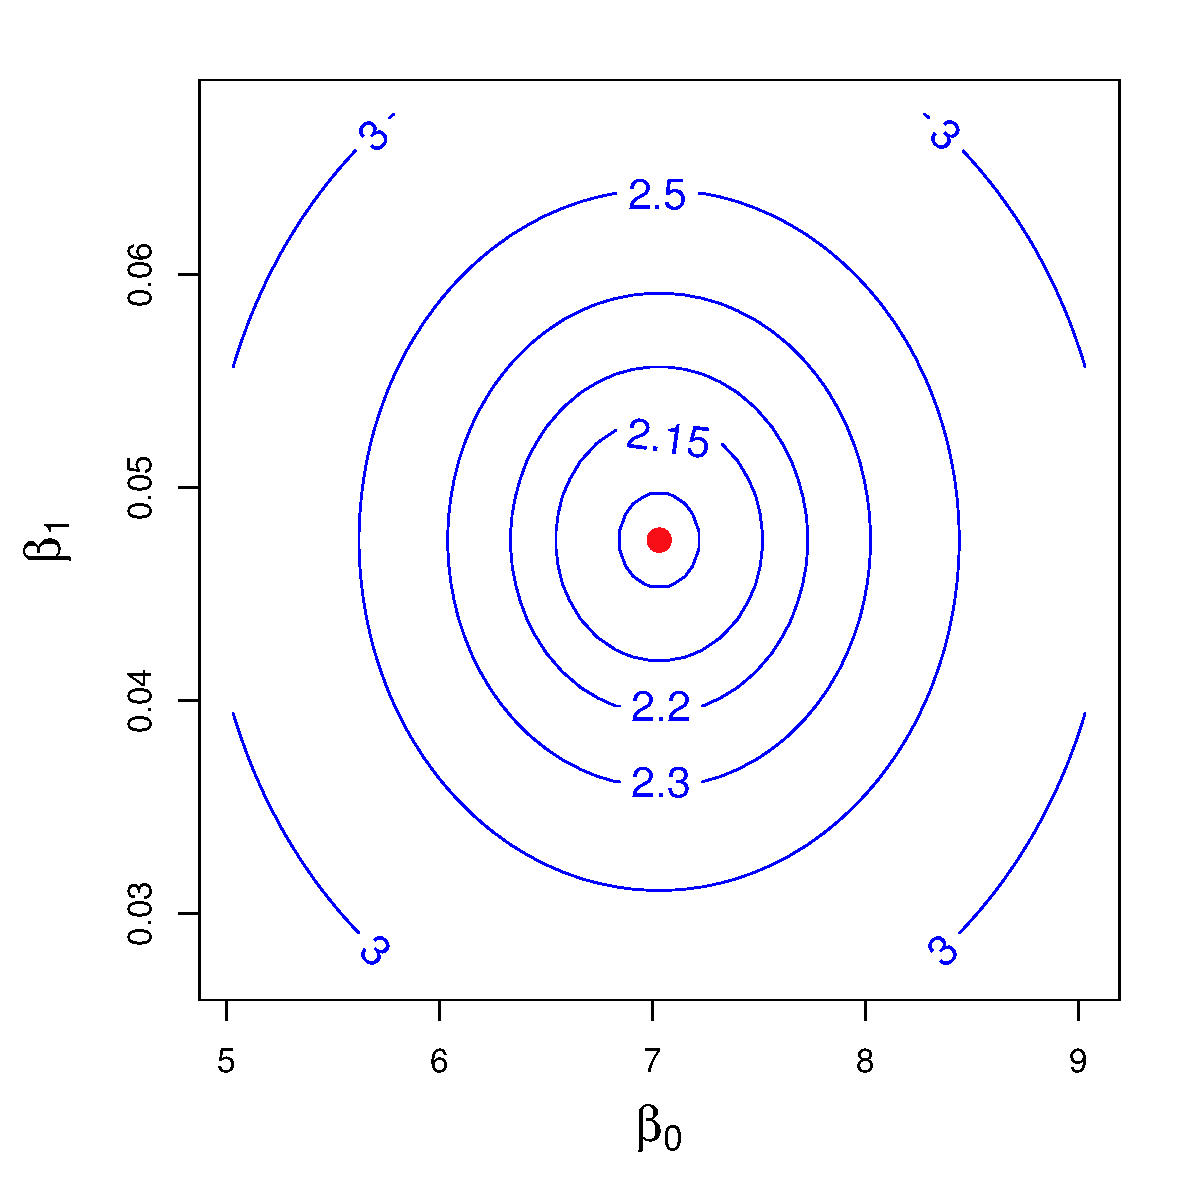
\includegraphics[width=0.4\textwidth]{3_2a}
		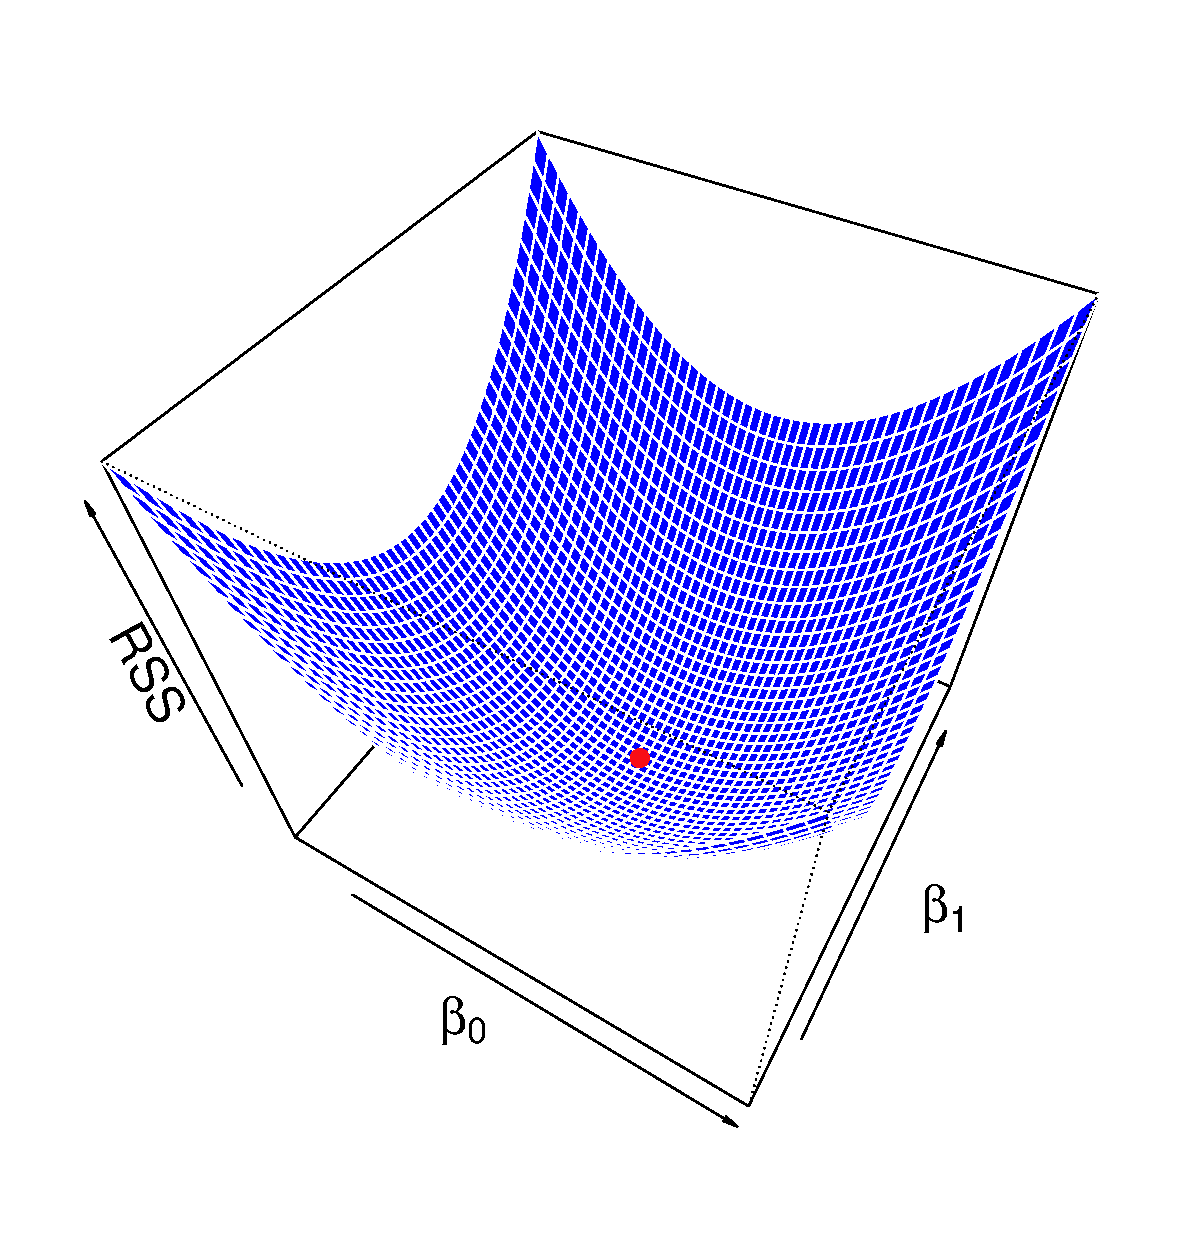
\includegraphics[width=0.4\textwidth]{3_2b}

		The RSS with \dat{sales} as the response and \dat{TV} as the predictor. The red dot marks the optimum.
	\end{center}
\end{frame}

\begin{frame}{Assessing Accuracies}
	\begin{itemize}
		\item We want to \e{quantitatively} answer two rather important questions: 
	\end{itemize}
	\begin{cpage}
		\begin{enumerate}
			\item \e{\orange Is there a relationship between the predictor and the response?}
			\item \e{\orange To what extend does our model fit the data?}
		\end{enumerate}
	\end{cpage}
	\begin{itemize}
		\item To this end, we need to clarify a few concepts. In particular the notions of \e{population},
			\e{sample} and \e{degrees of freedom}.
		\item Then we introduce a number of so-called \e{statistics}. Simply put, these are useful quantities
			we can compute from our data.
		\item It is beyond the scope of this course to formally justify all of this, but we will now
			spend some time to develop some intuition.
	\end{itemize}
	\bottomline{For this interlude we will look at the simpler problem of estimating a mean.}
\end{frame}

\begin{frame}{Populations}
	\begin{itemize}
		\item We (somewhat sloppily) define a \e{population} as the \e{full set} of potential observations.
		\item That could be an actual population (as in everyday language) like, say, the population\\
			of \e{all} \href{https://en.wikipedia.org/wiki/Blue\_whale}{\blue\underline{blue whales}} 
			alive on Earth today.
		\item It can also be the full set of instances of any abstract entity.
		\item We then might be interested in measuring a certain property of the instances in the population.
		\item For example, the \dat{length} of all blue whales alive on Earth today.
		\item Often we want to summarise our findings rather than presenting a raw data table \\
			(or graphical representation thereof). 
		\item A common way to summarise the data is reporting the \e{mean} and the\\
			\e{standard error} of the quantity of interest.
	\end{itemize}
	\bottomline{Note that there is nothing wrong with reporting the full distribution!}
\end{frame}

\begin{frame}{Samples}
	\begin{itemize}
		\item In practice, it is generally not possible to access the whole population.
		\item Quite literally, we don't have access to \e{all} blue whales.
		\item But we can look at a \e{sample} of the full population.
		\item The sample is a subset of the population we have access to.
		\item We generally assume the sample to be a \e{random sample}.
		\item Then we can try to \e{estimate} the mean and variance of the quantity of interest\\
			from the sample.
		\item Clearly, our estimates will \e{not} yield the \e{true} values of the mean and the variance.
	\end{itemize}
	\bottomline{Our goal is to avoid any \e{bias} in the estimates and evaluate their \e{accuracy}.}
\end{frame}

\begin{frame}{Estimating the Population Mean}
	\begin{itemize}
		\item If we had access to the whole population we could calculate the \e{true} mean $\mu$.
		\item Sadly, we have only access to a sample of $n$ observations of the random variable $Y$.
		\item So all we can do is produce an estimate $\hat{\mu}$:
			\[ \hat{\mu} = \sum_{i=1}^n y_i \]
		\item This is the best possible \e{unbiased} estimate we can draw from a random sample.
		\item Intuitively, this is obvious from the fact that $\hat{\mu} = \mu$ if the sample covers
			the entire population.
	\end{itemize}
	\bottomline{It is \e{very} important that the sample is random. Beware of \e{selection bias}!}
\end{frame}

\begin{frame}{The Error of the Mean}
	\begin{itemize}
		\item Let's assume our sample was drawn from a normal (Gaussian) distribution with\\
			\e{unkown} mean $\mu$ but \e{known} variance $\sigma^2$.
		\item Then the squared \e{standard error} of our estimate $\hat{\mu}$ is:
			\[ \text{Var}(\hat{\mu}) = \text{SE}(\hat{\mu})^2 = \frac{\sigma^2}{n} \]
		\item It is then common to report our findings in the form 
			\[ \mu = \hat{\mu} \pm \frac{\sigma}{\sqrt{n}} \]
			or give a specific \e{confidence interval}.
	\end{itemize}
	\bottomline{In pratice we are rarely that lucky.}
\end{frame}

\begin{frame}{Estimating the Population Variance}
	\begin{itemize}
		\item More often than not, neither the population mean $\mu$ nor the variance $\sigma^2$ are kown.
		\item Then we have to leverage the the sample mean $\hat{\mu}$ to compute the \e{sample variance}
			\[ 
				\hat{\sigma}^2 = \langle (y_i - \hat{\mu})^2 \rangle 
				= \frac{1}{n}\sum_{i=1}^{n}  (y_i - \hat{\mu})^2
			\]
			as an estimate of the true population variance.
	\end{itemize}
	\bottomline{Unfortunately, this $\bm{\hat{\sigma}^2}$ is \e{biased} because in general $\bm{\hat{\mu} \ne \mu}$!}
\end{frame}

\begin{frame}{The Sample Variance Bias}
	\begin{columns}
		\begin{column}{0.7\textwidth}
			\begin{itemize}
				\item We have simulated a data set of blue whale \dat{length}s.
				\item The sample mean is $\hat{\mu} = 26.0$.
				\item The sample variance is:
					\[ \frac{1}{n} \sum_{i=1}^n (y_i - {\blue\hat{\mu}})^2 = 17.37 \]
				\item The \e{true} sample variance is (in general we don't have access to $\mu$): 
					\[ \frac{1}{n} \sum_{i=1}^n (y_i - {\orange \mu})^2 = 23.97 \]
			\end{itemize}
		\end{column}
		\begin{column}{0.3\textwidth}
			\begin{popblock}{0.95\textwidth}{{\blue $\hat{\mu}=26.0$}\\{\orange $\mu=22.5$}\\{\dark $n=5$}}
				\begin{tabular}[h]{lr}
					observation & \dat{length}\\
					1 & 24.23 \\
					2 & 29.57 \\
					3 & 25.14 \\
					4 & 30.10 \\
					5 & 20.97 \\
				\end{tabular}
			\end{popblock}
		\end{column}
	\end{columns}
	\bottomline{The sample variance is \e{systematically biased} to lower values.}
\end{frame}

\begin{frame}{Source of the Sample Variance Bias}
	\begin{itemize}
		\item The source of the bias is that the estimate $\hat{\mu}$ does \e{not} have $n$
			\e{degrees of freedom}.
		\item Intuitively, this can be understood from the extreme case of $n=1$.
		\item With $n=1$ the sample variance would be zero, resulting in a zero standard error.
		\item Clearly it does not make sense to assume absolute confidence in $\hat{\mu}$.
		\item We need \e{at least two observations} to even start estimating the standard error
			of $\hat{\mu}$.\\
			(If we don't know the true $\mu$, which is generally the case).
		\item We therefore apply
			\href{https://en.wikipedia.org/wiki/Bessel\%27s_correction}{\blue\underline{Bessel's correction}} 
			when computing the estimate $\hat{\sigma}^2$:
			\[ \hat{\sigma}^2 = \frac{1}{\orange n-1}\sum_{i=1}^n (y_i - \hat{\mu})^2 \]
	\end{itemize}
	\bottomline{For large $\bm{n}$ this distinction is less relevant. The idea extends to more than one parameter.}
\end{frame}

\begin{frame}{The Population Regression Line}
	\begin{itemize}
		\item Recall that the \e{true} relationship between $X$ and $Y$ takes the general form
			\[ Y = f(X) + \epsilon \]
			where $\epsilon$ is a random error term with mean zero.
		\item If we approximate $f$ as a linear function the relationship becomes:
			\[ Y = \beta_0 + \beta_1 X + \epsilon \]
		\item The error term is a catch-all for what we miss with this simplified model.
		\item This linear model defines the \e{population regression line}.
		\item This the best linear approximation to the true relationship between $X$ and $Y$.
		\item It is analogous to the \e{population mean} we discussed earlier.
	\end{itemize}
	\bottomline{Note that the true relationship is \e{not} required to be linear.}
\end{frame}

\begin{frame}{The Population Regression Line}
	\begin{center}
		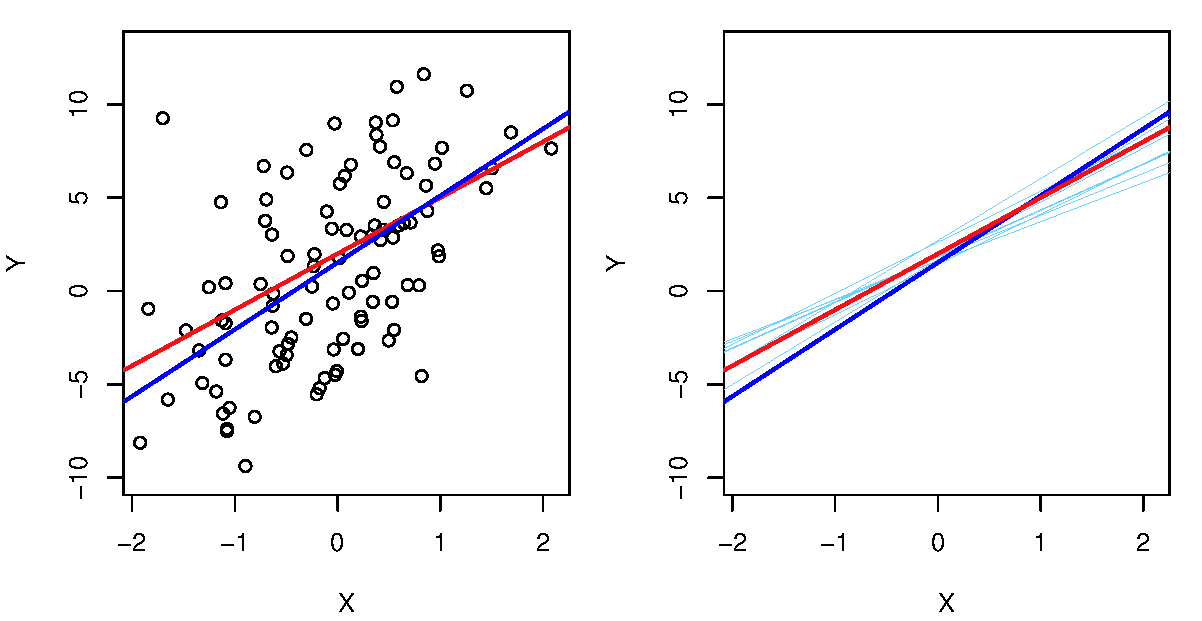
\includegraphics[width=0.6\textwidth]{3_3}
	\end{center}
	\vspace{-5mm}
	\begin{itemize}
		\item We created a random sample from the model $Y = 2 + 3 X + \epsilon$.
		\item The population regression line is shown in red.
		\item \e{Sample regression lines} are shown in blue.
	\end{itemize}
	\bottomline{The mean over many samples is close to the population regression line.}
\end{frame}

\begin{frame}{Accuracy of the Coefficient Estimates}
	\begin{itemize}
		\item The \e{sample regression line} is given by 
			\[ Y = \hat{\beta}_0 + \hat{\beta}_1 X \]
			with the estimated coefficients $\hat{\beta}_0$ and $\hat{\beta}_1$.
		\item The associated standard errors are then (this is a bit tedious to show):
			\[
				\text{SE}(\hat{\beta}_0)^2 = \sigma^2 \left( \frac{1}{n} + \frac{\overline{x}^2}{\sum_{i=1}^n (x_i - \overline{x})^2}\right)
				,\;\;
				\text{SE}(\hat{\beta}_1)^2 = \frac{\sigma^2}{\sum_{i=1}^n (x_i - \overline{x})^2}
			\]
		\item This assumes the $\epsilon_i$ are uncorrelated with variance $\sigma^2$.
	\end{itemize}
	\bottomline{In general the population variance $\bm{\sigma^2}$ is not known.}
\end{frame}

\begin{frame}{Estimating the Population Variance}
	\begin{itemize}
		\item If we don't know the population variance $\sigma^2$ we need to estimate it.
		\item This works like in the simple case of estimating a population mean.
		\item The estimated $\hat{\sigma}^2$, or \e{residual standard error}, is
			\[
				\hat{\sigma}^2 = \text{RSE} = \sqrt{\frac{1}{\orange n - 2} \text{RSS}}
				= \sqrt{\frac{1}{\orange n-2} \sum_{i=1}^n (y_i - \hat{y}_i)^2}
			\]
			with the \e{residual sum of squares}
			\[
				\text{RSS} = \sum_{i=1}^n (y_i - \hat{y}_i)^2
			\]
	\end{itemize}
	\bottomline{Note that number of degrees of freedom is now $\bm{n-2}$!}
\end{frame}

\begin{frame}{Confidence Intervals}
	\begin{itemize}
		\item Given the standard errors for the coefficient estimate, we can compute \e{confidence intervals}.
	\end{itemize}
			\begin{cpage}\orange
				A 95\% confidence interval is a range of values such that the interval will contain
				the true parameter value with a probability of 95\%.
			\end{cpage}
	\begin{itemize}
		\item This is a somewhat sloppy but very practical definition.
		\item In simple linear regression the 95\% confidence interval for the parameters $\beta$ is
			approximately:
				\[ \hat{\beta} \pm 2\cdot\text{SE}(\hat{\beta}) \]
		\item That is, with 95\% probability the true value $\beta$ lies in the interval
			\[
				\left[ \hat{\beta} - 2\cdot\text{SE}(\hat{\beta}),  \hat{\beta} + 2\cdot\text{SE}(\hat{\beta})\right]
			\]
	\end{itemize}
	\bottomline{This assumes Gaussian errors and large $\bm{n}$. In practice we use computers to get it right.}
\end{frame}

\begin{frame}{Hypothesis Testing}
	\begin{itemize}
		\item We are interested in whether $X$ is related to $Y$.
		\item This question is answered by a \e{hypothesis test}.
		\item Most commonly, we want to distinguish the \e{null hypothesis}
			\[ H_0 : \beta_1 = 0 \]
			from the \e{alternative hypothesis}
			\[ H_a : \beta_1 \ne 0 \]
		\item If $\beta_1 = 0$ then $Y = \beta_0 +\epsilon$ and there is no relationship between
			$X$ and $Y$.
		\item If $|\beta_1|$ is large, we can conclude that there is a relationship.
	\end{itemize}
	\bottomline{We need to quantify what we mean by ``large'' in this context.}
\end{frame}

\begin{frame}{The $\bm{t}$-statistic}
	\begin{itemize}
		\item Clearly, simply checking whether $\hat{\beta}_1 \ne 0$ is not good enough.
		\item The answer must depend on our confidence in the estimated value.
		\item This confidence depends on the value of the standard error $\text{SE}(\hat{\beta}_1)$.
		\item The \e{$t$-statistic} weighs the deviation of $\hat{\beta}_1$ from zero by the
			standard error:
			\[ t = \frac{\hat{\beta}_1 - 0}{\text{SE}(\hat{\beta}_1)} \]
		\item If there is \e{truly} no relationship between $X$ and $Y$, this quantity follows a\\
			\href{https://en.wikipedia.org/wiki/Student\%27s_t-distribution}{\blue\underline{$t$-distribution}}
			with $n-2$ degrees of freedom.
	\end{itemize}
	\bottomline{The $\bm{t}$-distribution approaches the normal distribution for large $\bm{n}$.}
\end{frame}

\begin{frame}{The $\bm{p}$-value}
	\begin{itemize}
		\item We can compute the probability to find a value of $|t|$ or larger from the $t$-distribution,
			assuming that there is truly no relationship between $X$ and $Y$.
		\item This probability is called the \e{$p$-value}.
		\item A high $p$-value indicates that we should accept the null hypothesis.
		\item A low $p$-value indicates we should reject the null hypothesis.
		\item Common values for rejecting the null hypothesis are $p < 0.05$ and $p < 0.01$.
	\end{itemize}
	\bottomline{Some disciplines require \e{much} lower $\bm{p}$-values to reject the null hypothesis.}
\end{frame}

\begin{frame}{Example: Advertising Data Set}
	\begin{popblock}{0.7\textwidth}{Regression of \dat{sales} onto \dat{TV}}
		\begin{tabular}[h]{lrrrr}
			{} & {\blue Coefficient} & {\blue Std. Error} & {\blue $t$-statistic} & {\blue $p$-value} \\
			\dat{Intercept} & 7.0325 & 0.4578 & 15.36 & $< 0.0001$ \\
			\dat{TV} & 0.0475 & 0.0027 & 17.62 & $< 0.0001$ \\
		\end{tabular}
	\end{popblock}
	\begin{itemize}
		\item We can reject $H_0 : \beta_0 = 0$ (that is, the mean of $Y$ is not zero).
		\item We can reject $H_0 : \beta_1 = 0$ (that is, \dat{TV} does influence \dat{sales}).
	\end{itemize}
	\bottomline{The probabilities of observing these values if $\bm{H_0}$ were true is virtually zero.}
\end{frame}

\begin{frame}{Model Accuracy}
	\begin{itemize}
		\item We now want to quantify the \e{extend to which the model fits the data}.
		\item For simple linear regression we use two quantities to do this.
	\end{itemize}
			\begin{cpage}
				\begin{enumerate}\orange
					\item The residual standard error, RSE.
					\item The $R^2$ statistic.
				\end{enumerate}
			\end{cpage}
	\begin{itemize}
		\item The RSE can be considered a measure of \e{lack of fit}.
		\item The $R^2$ statistic can be considered a normalised measure of the quality of fit.
		\item $R^2$ always takes on values between 0 and 1. It is independent of the scale of $Y$.
	\end{itemize}
	\bottomline{The $\bm{R^2}$ statistic represents the \e{proportion of variance explained}.}
\end{frame}

\begin{frame}{The $\bm{R^2}$ Statistic}
	\begin{itemize}
		\item The $R^2$ statistic is defined as
			\[ R^2 = \frac{\text{TSS} - \text{RSS}}{\text{TSS}} = 1 - \frac{\text{RSS}}{\text{TSS}} \]
			with the \e{total sum of squares}  
			\[ \text{TSS} = \sum_{i=1}^{n} (y_i - \overline{y})^2 \]
		\item We can think of the TSS as the total variance of the response $Y$ before\\
			the regression is performed.
		\item An $R^2$ close to zero indicates the regression does not explain much of the variability.
		\item An $R^2$ close to one indicates the regression explains a lot of the variability.
	\end{itemize}
	\bottomline{$\bm{R^2}$ measures the proportion of variability in $\bm{Y}$ that can be explained by $\bm{X}$.}
\end{frame}

\begin{frame}{Example: Advertising Data Set}
	\begin{popblock}{0.5\textwidth}{Regression of \dat{sales} onto \dat{TV}}
		\begin{tabular}[h]{ll}
			Residual standard error & 3.26 \\
			$R^2$ statistic & 0.612 \\
		\end{tabular}
	\end{popblock}
	\begin{itemize}
		\item On average, \dat{sales} deviate by 3,260 units from the regression line.
		\item The $R^2$ indicates that just under two thirds of the variability in \dat{sales} is explained\\
			by the regression onto \dat{TV}.
	\end{itemize}
	\bottomline{The $\bm{R^2}$ tells us that the simple linear regression model is reasonable.}
\end{frame}

\begin{frame}[plain]
	\begin{center}
		\href{https://xkcd.com/1132/}{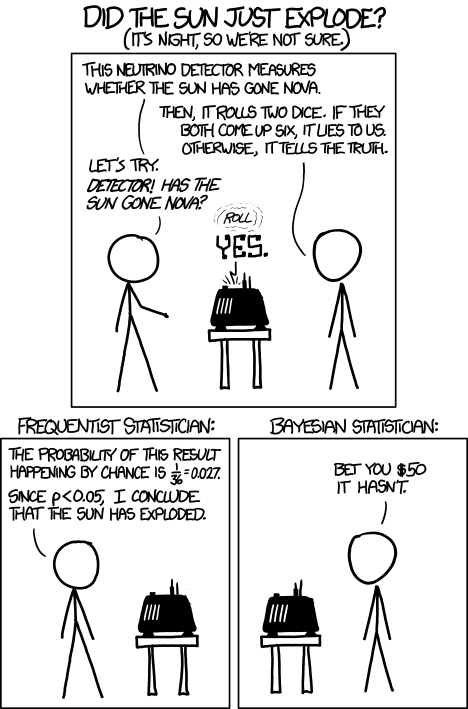
\includegraphics[width=0.35\textwidth]{l3/xkcd1132}}
	\end{center}
\end{frame}

\end{document}
